\documentclass[12pt,oneside]{report}

% ---------- Packages ----------
\usepackage[utf8]{inputenc}
\usepackage[T1]{fontenc}
\usepackage{times}
\usepackage{mathptmx}
\usepackage{setspace}
\usepackage{geometry}
\geometry{letterpaper, margin=1in}
\usepackage{graphicx}
\graphicspath{{figures/}}
\usepackage{caption}
\usepackage{subcaption}
% ML conference style captions
\captionsetup{font=small, labelfont=bf, skip=8pt}
\captionsetup[sub]{font=footnotesize, labelfont=bf}
\usepackage{booktabs}
\usepackage{amsmath, amssymb}
\usepackage[hidelinks]{hyperref}
\usepackage[nameinlink,capitalise]{cleveref}
\usepackage{enumitem}
\usepackage{xcolor}
\usepackage{titlesec}
\usepackage{xparse}
\usepackage{xspace}
\usepackage{mysymbols}

% Minimal approach - let LaTeX handle TOC normally
\usepackage{csquotes}
\usepackage[style=numeric-comp,natbib=true,sorting=none]{biblatex}


\NewDocumentCommand{\scsurname}{m m o}{%
  #1~\textsc{#2}%
  \IfValueT{#3}{\space #3}%
}

\addbibresource{references.bib}

\setcounter{secnumdepth}{3}
\setcounter{tocdepth}{2}
\setstretch{1.15}

% Custom chapter formatting - remove "Chapter" prefix and newlines
\titleformat{\chapter}[hang]
{\normalfont\Large\bfseries}{\thechapter}{1em}{}
\titlespacing*{\chapter}{0pt}{0pt}{15pt}

% Tighter section spacing
\titlespacing*{\section}{0pt}{12pt plus 2pt minus 2pt}{8pt plus 2pt minus 2pt}
\titlespacing*{\subsection}{0pt}{10pt plus 2pt minus 2pt}{6pt plus 1pt minus 1pt}

% ML conference style paragraph formatting
\setlength{\parindent}{0pt}
\setlength{\parskip}{6pt plus 2pt minus 1pt}

% ---------- Convenience ----------
\newcommand{\todo}[1]{\textcolor{red}{TODO: #1}}
\DeclareRobustCommand{\etal}{\emph{et~al.}\xspace}

% ---------- Title Info ----------
\newcommand{\proposaltitle}{Deep Learning for Scalable Sensorimotor Brain-Computer Interfaces}
\newcommand{\authorname}{Joel Ye}
\newcommand{\department}{
  Neural Computation, Neuroscience Institute \\
  Machine Learning Department, School of Computer Science \\
}
\newcommand{\university}{Carnegie Mellon University \\ Pittsburgh, PA}
\newcommand{\proposaldate}{July 30, 2025}

\newcommand{\committee}{%
  \scsurname{Robert}{Gaunt}[({co-chair})]\\[0.15\baselineskip]
  \scsurname{Leila}{Wehbe}[({co-chair})]\\[0.15\baselineskip]
  \scsurname{Jennifer}{Collinger}\\[0.15\baselineskip]
  \scsurname{Aran}{Nayebi}\\[0.15\baselineskip]
  \scsurname{Chethan}{Pandarinath}[({Emory University})]%
}

% ---------- Document ----------
\begin{document}

% --- title page ---
\begin{titlepage}
\setlength{\parindent}{0pt}
\centering

% top breathing room
\vspace*{\stretch{1}}

% Title block
{\LARGE\bfseries \proposaltitle\par}
\vspace{0.6\baselineskip}
{\Large \authorname\par}

\vspace{1.5\baselineskip}
{\large PhD Thesis Proposal\par}
{\small \proposaldate\par}

\vspace{1.2\baselineskip}
{\normalsize
\begin{minipage}{0.9\textwidth}\centering
\department
\university
\end{minipage}\par}

% middle breathing room (larger to push committee lower)
\vspace*{\stretch{2}}

% Committee block
{\large\bfseries Thesis Committee:\par}
\vspace{0.4\baselineskip}
{\normalsize
\begin{minipage}{0.7\textwidth}\centering
\setlength{\parskip}{0pt}%
\committee
\end{minipage}\par}

% bottom breathing room (largest to anchor footer)
\vspace*{\stretch{3}}

{\small\itshape
Submitted in partial fulfillment of the requirements for the Degree of Doctor of Philosophy\par}

\vspace*{\stretch{1}}
\end{titlepage}
\pagenumbering{arabic}

\section*{Abstract}
\addcontentsline{toc}{section}{Abstract}
The increasing ambition of neuroscience and neurotechnology both supplies and demands vast new quantities of neural data, which creates a critical need for methods that can operate effectively on neural data at scale.
This need could potentially be addressed by deep learning (DL).
Here, we assess this program for sensorimotor intracortical brain-computer interfaces (iBCI). iBCI systems have traditionally been built by collecting short datasets to relate a user’s neural activity with their bodily state. Although this approach can enable both motor control and sensory feedback in research settings, iBCI's real-world adoption will further depend on achieving high performance with exquisite reliability and convenience. In other words, iBCI systems must, too, evolve to operate effectively on BCI data at real-world scales.
To this end, I present one completed study and two proposed projects that show how deep learning models can provide a platform for scaling BCI systems. Through this platform, I promote the view that BCI models can and should be built to reflect the BCI system's lifelong data collection.

% Therefore, this challenge might be best met with deep learning models that encapsulate the landscape of data accumulated throughout the BCI device's lifetime.
% Therefore, this challenge might be best met with deep learning models that encapsulate the landscape of data accumulated throughout the BCI device's lifetime.
% deep learning becomes an  provide a tractable platform with which to encapsulate this landscape.
% That is, by reframing the accumulation of BCI datasets throughout device lifetime not as standalone snapshots but as a landscape of related data,
%  reframe BCI data not as a collection of standalone datasets but as a store of related data accumulated throughout the BCI device's lifetime.
% I next introduce one result and two proposed works that build this case.

\textbf{Aim 1: Large scale pretraining improves modeling of intracortical motor datasets [in submission].}

The driver of deep learning’s efficacy across domains is its ability to leverage conserved statistical structure across datasets, primarily enabled by a stage of model preparation on large scale data called pretraining. Previous work has identified the requisite conserved structures across motor cortical datasets, and so we systematically measure the efficacy of deep neural network (DNN) pretraining on such datasets. We establish that DNN efficacy improves with neural data scale on both multi-subject and multi-behavior datasets. Yet, this scaling has diminishing returns as data in the downstream, target setting grows, rendering the scaling less impactful for long term BCI applications. We conclude that pretrained networks may accelerate initial BCI calibration speeds but will not fundamentally remove the need for continuous BCI data collection.

\textbf{Aim 2: Pretrained deep networks enable rapid and scaleable upper limb neuroprosthetic control [proposed].}

High degree of freedom control of a robotic arm and hand is possible with current iBCIs, but requires extensive daily recalibration and experimenter intervention. Based on successful deep network use in speech BCIs, we propose that an NDT-based controller which accumulates calibration data across days can address both of these challenges. We will evaluate NDT for 7-degree of freedom neuroprosthetic upper limb control in up to two human participants, aiming to demonstrate rapidly calibrated robotic upper limb control. We further aim to demonstrate the model’s scalability by extending this control to additional degrees of freedom in the hand without changes to the model design.

\textbf{Aim 3: Surveying the neural response to intracortical microstimulation [proposed].}

Sensory feedback is integral to native motor control, and can be provided in iBCIs through intracortical microstimulation (ICMS) of the somatosensory cortex. Yet, current characterization of different ICMS patterns relies nearly entirely on expensive and noisy behavioral reports, instead of through its impact on ongoing neural activity. A predictive model of the neural response to ICMS is needed to accelerate the development of sophisticated ICMS protocols. Towards this goal, we first introduce a method to recover spiking activity from artifacted recordings, and then taxonomize the sensory neural response to ICMS through transfer learning experiments. In this taxonomy, we show that the neural response to temporally varied stimulation shares transferable structure, but responses across different stimulation channels are much more idiosyncratic. These results inform the design of protocols to accurately map the neural response to ICMS.

% Table of contents
\tableofcontents

\cleardoublepage

% =========================
% Introduction
% =========================
\chapter{Introduction and Background}

\begin{figure}[h]
  \centering
  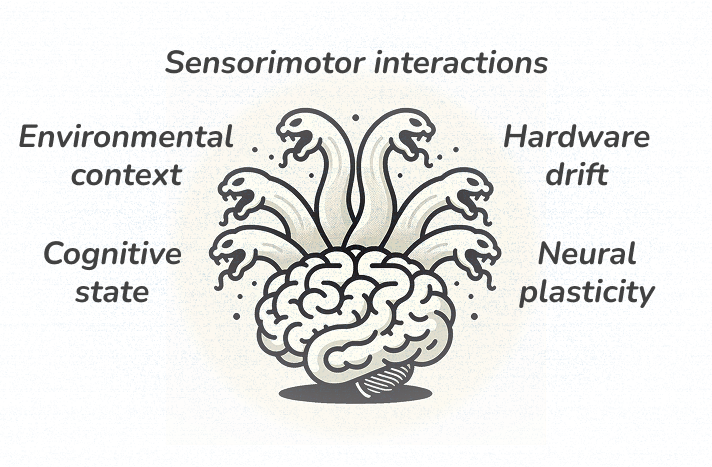
\includegraphics[width=0.9\linewidth]{ch1_hydra.png}
  \caption{Models of neural data must robustly relate neural activity to certain variables of interest while accounting for the influence of numerous other factors that also modulate the same neural activity.}
  % \caption{The role of a computational model is to provide an interface to interact with the underlying domain data. A scalable model is one that provides a tractable strategy to encapsulate and query a growing variety of data.}
  \label{fig:hydra}
\end{figure}

Today, neuroscientists seek to study the brain in natural, dynamic environments, and neurotechnology companies are similarly racing to produce a device that will work robustly in the real world.
In this increasing scope, a great variety of factors can affect the neural data that BCI devices collect, and consequently, the performance of the models built on that data. In the best cases, we have some mechanistic account of these factors, such as in our characterization of the physical degradation at the neural-electrode interface~\citep{pandarinath_22_review,bjaanes2024quantifying}. In other cases, well-controlled experiments provide a strong descriptive characterization, as in the case of cognitive states~\citep{cowley2020slow,smoulder2024neural} and body posture~\citep{marino2024posture}. Most often, we lump the remaining factors in the catch-all term of ``context,'' as often arises in studying similar motor behaviors under variable task requirements~\citep{mender23ctx,ma2021ctx,downey2017object}. Designing BCI systems that perform at scale is thus daunting because it should require accounting for all of these known factors and presumably many more unknown ones.

Fortunately, progress in BCIs has rarely hinged on theoretical clarity. The first population vector decoders were enabled by the observation that motor neurons fired reliably according to cosine tuning curves~\citep{Georgopoulos1986}, not from a mechanistic understanding of why they did so. A caricatured workflow for mitigating the myriad impacts of the above factors is to collect data and use this data to update our models. A deeper understanding can support expectations of model robustness, but ultimately, we must design BCIs that recover gracefully when our understanding eventually fails. Likely, the rate of BCI progress will hinge on how quickly our methods can adapt to empirical failures as they arise.

To minimize the Sisyphean burden of this task, many domains faced with similar challenges have turned to deep neural networks, deprioritizing interpretable theories in favor of radical empiricism~\citep{wang2023scientific}. In this proposal, I aim to establish such a data-driven framework for thinking about sensorimotor BCIs, describing three ways in which we can use deep networks to relate and aggregate BCI datasets. To contextualize this work, I will introduce brain computer interfaces and deep learning’s application to BCIs in turn.

\section{Brain-computer interface models}
\label{sec:bci_models}

\begin{figure}[h]
  \centering
  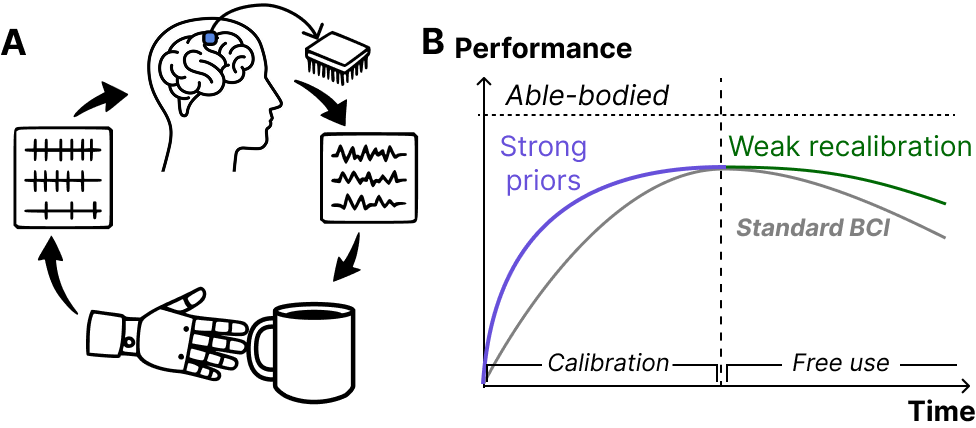
\includegraphics[width=0.95\linewidth]{ch1_loop_and_lifecycle.png}
  \caption{A) A sensorimotor BCI-enabled control loop. By recording neural activity from an implanted microelectrode array, this BCI can allow the user to control a robotic hand. When touch sensors on the hand contact a physical object, we can deliver stimulation pulses back to the brain to provide the user sensory feedback. B) Motor BCI models must be calibrated to relate neural activity at the implant interface with the user's intentions. Performance increases over an explicit calibration phase, which can be accelerated with learned priors, but will decline over time during free use of the system. This decline can be mitigated with varied recalibration methods.}
  \label{fig:bci_overview}
\end{figure}

A brain-computer interface (BCI) is a system that allows observation and control of neural activity. In the rehabilitative setting, for example, BCIs can record from motor cortex to predict movement intentions and can control sensory cortex to evoke sensations. Together, the premise of a sensorimotor BCI is that we might directly relate a user's neural activity with their sensorimotor experience, and thereby restore a degree of sensorimotor function to a paralyzed user~(\figref{fig:bci_overview}A).

Over the last two decades, a number of studies have demonstrated the efficacy of human BCIs based on implanted microelectrode arrays~\citep{Brandman17Review,pandarinath_22_review}.
With implants in motor cortex recording neuronal spiking activity, users have achieved control of digital cursors, robotic arms, and language and speech generation~\citep{collinger2013high,willett_23_speech,wairagkar25voice,Pandarinath2017Pointandclick}.
With stimulation of implants in somatosensory cortex, users perceive tactile sensations on their hand, which is valuable as an end in itself but can also be utilized functionally for more skillful motor control~\citep{flesher2016intracortical,graczyk2024clinical,flesher2021functional,ArmentaSalas2018}.
BCI algorithms research now unfolds on several axes, naturally including expanding BCI capabilities to new functional milestones~\citep{willsey2024real,wairagkar25voice}, but also making the existing repertoire reliably performant across users and time~\citep{hosman2023months,fan2023plugandplay}, and minimizing user burden for system adoption~\citep{pandarinath_22_review,card2025long}.

\textbf{Motor BCI challenges}: Motor innovations can be organized by evaluating impact to BCI performance over time~(\figref{fig:bci_overview}B). BCI models are initialized with a calibration protocol where experimenters collect by paired neural activity and motor intention labels by prompting the user to behave according to experimental cues. The gray arc shows how BCI performance will increase with this calibration period~\citep{makin_18_refh}, but then decline over time due to signal nonstationarities that render the calibration data less relevant~\citep{karpowicz2022stabilizing}. Performance gain from calibration can be accelerated with strong priors, and given that practical constraints often end calibration before performance saturation, such priors may improve attained performance. Next, preserving model performance over time is a major priority for real world convenience, as the worst case strategy of recalibrating models from scratch imposes substantial user burden. One strategy to achieve persistent performance is collect a large corpus of calibration data across multiple days. This strategy has been used to provide multiple months of continuous performance in speech BCIs and 2D cursor control BCIs~\citep{willett_23_speech,card2024accurate,sussillo_16_future,hosman2023months}. Performance can also be explicitly maintained by using minimal supervised recalibration or behavioral priors (Weak recalibration)~\citep{wilson_23_prit,fan2023plugandplay}.
Multi-day data modeling has also enabled stable reach and grasp performance in an electrocorticographic (ECoG) device~\citep{Natraj2025robot}, but has not yet been applied for high performance simultaneous multi-DoF upper limb control.

\textbf{Sensory BCI challenges}: In contrast, sensory BCIs currently struggle less in model stability and more in building precise models of evoked sensations to begin with. That is, while any given stimuli's evoked percept location and quality appear relatively stable over time~\citep{greenspon_25_stable}, how these features of the evoked sensations relate to electrode choice and stimulation parameters are difficult to predict~\citep{hughes2021perception}. The consequence is that sensory BCI capabilities are currently developed by collecting a library of responses to varied stimulation patterns and selecting a subset of relevant patterns for use in functional tasks. One promising framework to guide future stimulation design is the principle of biomimicry. Biomimetic ICMS asserts that stimulation should be designed to evoke neural responses resembling those of natural touch, rather than directly matching stimulation frequencies or amplitudes to physical parameters~\citep{bensmaia2023restoration}. However, this aspiration is hamstringed on both ends, as it is difficult both to observe the neural response to ICMS and to observe the neural response to natural touch in BCI participants who typically have impaired somatosensory pathways. Current demonstrations of biomimetic ICMS have compromised by matching coarse, subject-general features of natural touch and assuming the neural response to ICMS is proportional to either frequency or amplitude inputs~\citep{valle2025tactile,hobbs2025biomimetic,greenspon_25_stable}. Realizing biomimetic ICMS in higher fidelity through neural activity, and thereby presumably improving somatosensory BCI efficacy overall, will require addressing both these assumptions.


\section{Deep network models of BCI data}
\label{sec:deep_networks}

Modern deep learning organizes applications research by the data being modeled, the model architecture, and the optimization objective. We will take this approach to introduce deep networks in BCI.

\textbf{Data}:
The neural data recorded from our BCIs are multichannel voltage timeseries. Most traditionally, and in the majority of this proposal, this broadband voltage will first be filtered and thresholded to extract rapid, transient deflections, which mark putative spikes from a neuron nearby the recording electrode. A typical BCI dataset will include 100 to 200 electrode channels of data with dozens of high amplitude spiking waveforms, along with many more channels recording multiunit activity that is is not easily seperable into distinctive waveforms. Our motor datasets will also contain upper limb covariates, for example in the form of kinematics or electromyography that varies on the timescale of seconds. In non-human primate (NHP) datasets, these behaviors generally derive from physical sensors, but as mentioned in~\secref{sec:bci_models}, a different strategy must be used to create human BCI datasets since human BCI users have impaired control of their native limb. Human BCI datasets instead assert a certain behavior and experimentally cue the user to attempt the behavior. This artificial association means that the behavior label is likely to be temporally warped and otherwise imprecise~\citep{merel2016neuroprosthetic} relative to the unobserved motor intention of the user.
%  We can also frame this process as a user labeling of the cued behavior data with their neural activity.
The electrical stimuli that we use in sensory datasets comprise trains of biphasic current-controlled pulses, where each individual pulse’s timing and amplitude can be varied. Perceptual reports to ICMS, to the extent discussed in this proposal, will be described in terms of binary detection or scalar ratings of intensity.

\textbf{Architecture}: The mainstays of broader deep learning architectures that have flourished in the last decade, including multi-layer perceptrons (MLPs)~\citep{Willsey2022HighVelocity}, convolutional neural networks (CNNs)~\citep{temmar2024artificial}, recurrent neural networks (RNNs)~\citep{pandarinath_18_lfads}, and Transformers~\citep{ye_21_ndt}, have all been applied to BCI data. Unlike in other domains, BCI has yet to reach consensus on the most performant architectures.
This proposal presumes the view of the Bitter Lesson~\citep{sutton2019}, which states that performance differences across architectures may be minor relative to gains from increasing data scale.
Adopting this view, we contrast here only the RNN, which many neuroscientists may have familiarity with, and the Transformer, which has empirically dominated the architectural landscape in machine learning (ML) domains, including even other timeseries domains like audio processing~\citep{radford2022whisper}. RNNs process timeseries data one timestep at a time, maintaining an internal state that evolves with the input data. An RNN provides an appealing interpretative lens for neural data, as its iterations describe the evolution of the neural dynamical system. The Transformer, in contrast, does not maintain a centralized state but instead learns the relationship between fragments of the data. Each of these fragments is called a token, and they could be for example the population activity vector at the start of an experimental trial, abstract metadata about the experiment, or the vertical velocity of a user’s arm.

\textbf{Objective}: This proposal focuses on predictive objectives, namely regression and classification. This will be true despite variety in the qualitative function of our different models. When the work’s objective is to model neural data in isolation, we say we are interested in the model’s representation learning. At other times, we say we are building decoders of neural data to predict behavior, or encoders of stimuli to predict neural activity. With the lens of deep networks in particular, these different terms all implementationally overlap, in that the underlying models are operating between one or two data modalities.

\textbf{Challenges}: BCI datasets feature a number of challenges that uniquely interact with deep learning. First, by experimental design, there is often a large component of the neural data that appears strongly connected to the covariate of interest, implying there is not an immediately clear role for nonlinear DNNs. For example, in the motor cortex, we can identify single neurons with firing activity that can be well characterized by a cosine tuning curve with two parameters, a preferred arm direction and depth of firing rate modulation to movement in that direction. To balance this simplicity, BCI datasets will often have nonstationarities~\citep{downey_18_stability,wimalasena2020unstable,perge2013intra}, as discussed in the introduction. New cognitive states, neurophysiological changes at the electrode interface, and BCI system hardware state can all introduce shifts in the observed activity. These externalities are difficult to directly observe, so we must build systems that are implicitly robust to these shifts so as to enable stable BCI performance~\citep{sussillo_16_future}.

\textbf{Foundation models}: A modern trend in deep learning applications research is to create a model that provides broadly competent performance across tasks in a field, at which point the model can be considered a ``foundation model''. Foundation models were most deservingly coined in the context of natural language processing (NLP)~\citep{bommasani2022opportunitiesrisksfoundationmodels}, where a large scale initial training phase (pretraining) across internet text created models that quickly dominated all mainstream benchmarks~\citep{brown2020languagemodelsfewshotlearners}.
Critically, model performance correlates reliably with the scale of pretraining, providing the impetus for many fields to also measure the empirical “scaling” of model performance with their own domain's data~\citep{kaplan2020scaling}.
The merit of this paradigm for neuroscience writ large is still under debate, but this has not deterred a number of different efforts to create these large models in BCI domains~\citep{dyer_richards_2025_bitter_lesson}. Aim 1 discusses precisely this effort for intracortical motor BCI data.

% \textbf{Deep learning as systems tools}: The practice of deep learning is distinguished from the broader machine learning discipline by its strong empiricist culture. Mantras on model behavior develop based on what has previously been effective, like focusing on data over models or focusing on broad task performance over single tasks~\citep{abnar2021exploringlimitslargescale}. One pertinent empirical view is that foundation models are at minimum a catalog of their training data, and can easily learn simple functions. The value of this capability is exemplified in text cleaning, a domain that systems researcher Christopher Ré describes as facing a death by a thousand cuts, where individual problems are not technically challenging but their breadth and non-enumerability frustrate systematic solutions. Remarkably, early language models (GPT3) provided a simple solution to sanitizing human text entry and documents for errant values, outperforming rules-based agglomerations that received years of investment. Similarly, neural data appears locally linear in any given context, and the neural population activity may in fact be neatly organized so that certain aforementioned nonstationarities may simply not degrade existing models. It would be foolhardy to expect this in generality, however, as simply across behaviors, the neural data distribution will begin appearing nonlinear~\citep{fortunato2024nonlinear}. It is thus through this systems lens that I most expect BCIs to benefit from deep learning.



% =========================
% Aim 1
% =========================
\chapter{Aim 1: Large-scale pretraining for intracortical neural datasets}

\section{Summary and Significance}

Deep learning’s greatest successes have depended on exploiting large and varied datasets. None of these efforts have occurred in a vacuum, but rather, have depended on the gradual scaling of model training and continual, critical evaluation. Growing the deep learning paradigm in neural data will also require quantifying the benefits from scaling the size and diversity of data used in model training. Fortunately, we approach this problem at a time when the neuroscience field has already identified structural relationships in data collected across time periods, subjects, and behavioral tasks, which delineate a natural scope for model training data.

We perform two scaling studies on Transformer pretraining across motor cortical datasets. In the first study, we measure the returns on increased pretraining data along the three aformentioned axes of data diversity. We find that, under the lens of the model we used, cross-session data scales nearly as well as data collected on the same day, and that cross-subject and cross-task data lag behind but still have productive returns to scaling. The second study executes on this premise, fitting a single large Transformer to 2000 hours of neural activity pooled from over 40 implanted monkeys and humans. Here, we see continued benefits from increasing pretraining data, but add the important caveat that benefits decline inversely with increasing data availability in deployment settings.

\textbf{Significance}: This work provides a baseline quantification of the benefit of scaling deep learning for motor cortical decoding, grounding narratives on currently feasible data scales and projecting returns on larger ones. To this end, we show that the standard expectations of pretraining are met, in that scaling up provides increased data efficiency in a broad class of new datasets. Moreover, the work dissects the distinct benefits of the different axes of neural data diversity, which all scaled pretraining on neural data must contend with. Under our Transformer models, each neural dataset has considerable individual variability, and transfer learning drops off greatly when using data from different subjects. Thus, while pretraining with up to 2000 hours of data is useful, it does not qualitatively reduce the data needed to achieve high performance in most downstream settings, and therefore does not fundamentally alter data collection strategies for high performance BCI.

\paragraph{Papers.}
\begin{itemize}
  \item Ye \etal, Neural Data Transformer 2. NeurIPS 2023.
  \item Ye \etal, A Generalist Intracortical Motor Decoder. (In submission)
\end{itemize}

\section{Approach}
The full pipeline needed to prepare foundation models like language models is complex beyond the scope of this proposal. Here, we study the earliest stage of model preparation, known as pretraining, and the pretrained model’s immediate adaptation to a new setting, known as fine-tuning. Pretraining requires the availability of some large and loosely related volume of datasets in the domain of interest, while fine-tuning assumes the availability of some small amount of data that is much more closely related to the evaluation data. For example, if we were to assess a language model’s ability to produce scientific-sounding text, the pretraining dataset might be all of Wikipedia, or all of the Internet’s language content, and the fine-tuning data may be given as an article from a recent journal. For neural data, we must shortly define what the loosely related pretraining data might mean relative to our target domain of intracortical human BCI. In fine-tuning, we use a random temporal subset of our actual evaluation datasets.

We aim to characterize the impact of both data and model design parameters on final model performance. In both pretraining and fine-tuning, the data varies qualitatively in how training data and evaluation data relate, and quantitatively in the training data volume. The deep learning literature identifies two model factors as critical in scaling studies: the number of parameters in the deep network model and the compute used in training the deep network.

\textbf{Data}: These studies use previously collected datasets that were either released publicly or internal to Rehab Neural Engineering Labs (RNEL) and our collaborators. Data varies in the lab and experimental hardware that was used for collection, in the NHP or human subject that produced the data, time period of collection, and behavior in the task. The behaviors largely comprise reaching and grasping from experimental paradigms containing short, repeated trials, but still contain large diversity in the number of experimental conditions and behavior sensors.


\begin{figure}[h]
  \centering
  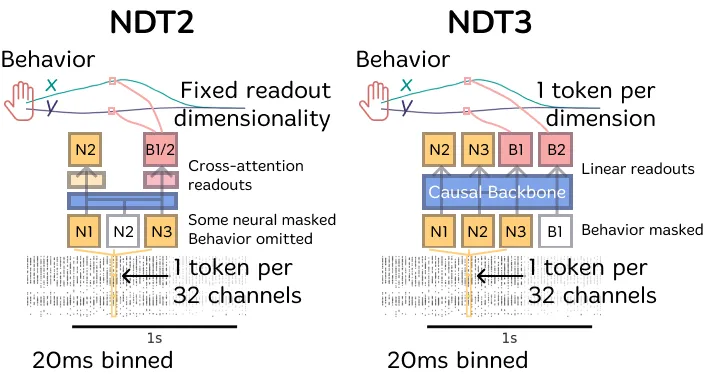
\includegraphics[width=0.8\linewidth]{ch2_ndt_models.png}
  \caption{NDT2 and NDT3 both take input neural data and output neural data and behavior predictions. Both models tokenize neural data in time with 20ms timebins and in space by dividing the population activity into subsets of fixed size (32 in this figure). NDT2 emits one behavior token for prediction at each timestep, while NDT3 emits one behavior token per behavior dimension and timestep, which enables streamlined prediction of behavioral data of varied dimensionality. NDT2, inspired by a Masked Autoencoder design~\citep{he_21_mae}, masks out a fraction of neural token inputs and only predicts this fraction. NDT3 adopts the autoregressive modeling framework and allows prediction of all neural tokens conditioned on neural tokens from previous timesteps. }
  \label{fig:ndt_models}
\end{figure}

\textbf{Models}: The great variety of datasets we aim to model at once in pretraining requires flexible model designs, as the identity and count of neurons in each dataset’s population activity will differ across datasets. Here we discuss models based on the Transformer to meet this challenge. In~\figref{fig:ndt_models}, we review the Transformer’s data processing in the specific contexts of the NDT2 and NDT3 architectures. The Transformer model requires input data to be fragmented into a number of tokens. Once these tokens are defined, they are simultaneously processed through a stack of alternating attention and MLP layers. Attention layers updates each token as a function of all tokens, while MLP layers update tokens individually. NDT’s major design obligation is to decide how to perform this tokenization. In both models, we tokenize spiking timeseries in time with a 20 ms binning operation, and in space with a patching operation. This patching operation divides the N-dimensional input, i.e. all electrodes in a subject, into groups of K channels, padding the input with zeros to resolve remainder channels. This design follows Transformers in computer vision, which similarly tokenizes 2D images into smaller patches of pixels~\citep{he_21_mae,dosovitskiy_2021_vit}. By analogy, smaller patches should increase model expressivity but incur increased computation and data requirements.

Note that the two model designs reflect their distinct motivations. NDT2 was developed to evaluate whether DNNs could learn transferable representations of neural spiking activity. It thus exclusively accepts neural data as input and extracts behavioral representations at each timestep with a linear layer of fixed output dimensionality. NDT3 was designed to accept highly variable data in order to scale pretraining as widely as possible. To do so, NDT3 accepts unidimensional behavioral tokens as inputs in order to specify how many behavior dimensions the model needs to predict.

\section{Results}


\begin{figure}[h]
  \centering
  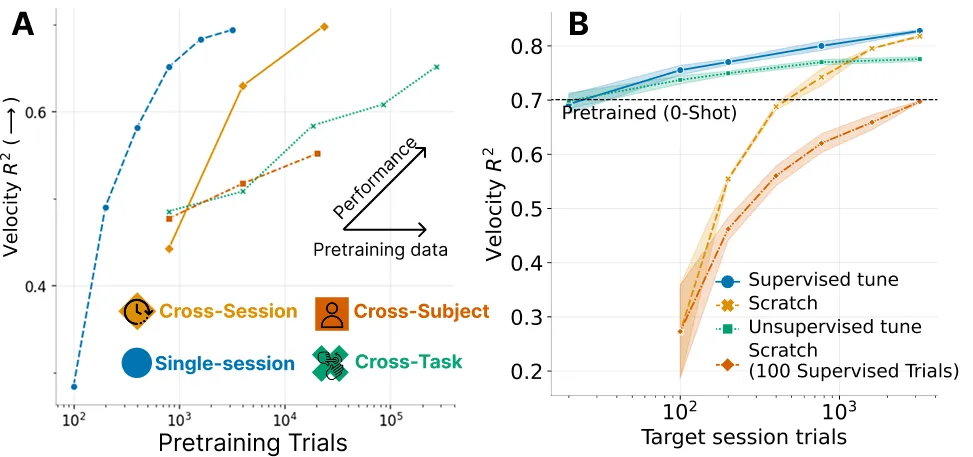
\includegraphics[width=0.8\linewidth]{ch2_ndt2_results.png}
  \caption{A. NDT2 decoding of monkey reach velocity scales with increasing pretraining data from different sessions, subjects, and behavioral tasks. The pretraining abscissa for the single-session curve indicates the total training data available to the model. For the order curves, the abscissa indicates the pretraining data scale. These pretrained models fine-tune to the target session with 100 trials of data. B. Pretrained multisession models can be deployed on new sessions for immediate zero-shot performance. They can also be tuned either through supervised or unsupervised objectives to improve performance, which outperforms models trained from scratch across tuning dataset size.}
  \label{fig:ndt2_results}
\end{figure}


NDT2 shows that DNNs can transfer learn across datasets of spiking activity from different sessions, subjects, and behaviors. Prior work to NDT2 demonstrated this transfer can be achieved with explicit mechanisms to align data from one setting to another, such as canonical correlation analysis~\citep{gallego_18_task} or joint training with alignment layers~\citep{pandarinath_18_lfads,turaga_13_stitch}. NDT2 demonstrates the same is possible merely through its population patching scheme. In subsequent experiments, we show the relative value of scaling pretraining trials from the different data sources, showing that cross-session data transfers much better than equivalently sized cross-subject or cross-task datasets~(\figref{fig:ndt2_results}A). Nonetheless, the positively scaling benefits from increased pretraining on all these varied datasets suggests that we should expect benefits from aggregating a large and diverse pretraining dataset.

\figref{fig:ndt2_results}B shows that a pretrained NDT2 model retains high performance for immediate use on a new day, without any data renormalization (0-shot). Further, NDT2 can be fine-tuned for a new day either through unsupervised or supervised calibration. This strategy outperforms models that are trained from scratch at all fine-tuning data scales, so the implication for BCI deployment is that pretraining should always be used when possible.

\begin{figure}[h]
  \centering
  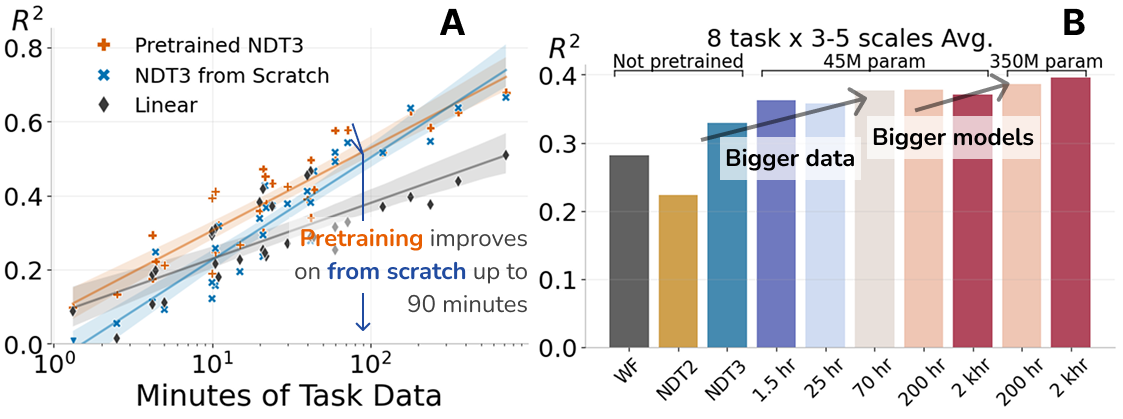
\includegraphics[width=0.8\linewidth]{ch2_ndt3_summary.png}
  \caption{NDT3 evaluations. \textbf{A}. When evaluations are organized by downstream data scale (Minutes of Task Data), a pretrained model is better than or equal to non-pretrained models and a linear baseline at all data scales. However, the non-pretrained NDT3 model matches the pretrained model when downstream task data is sufficiently large, here at 90 minutes. \textbf{B}: Collapsing all evaluations into a single average, we see that scaling pretraining dataset size and model size improves summary performance.}
  \label{fig:ndt3_summary}
\end{figure}


NDT3 builds on NDT2’s scaling results and pretrains Transformers on up to 2000 hours of motor cortical spiking activity and behavior. We conduct an evaluation commensurate with this pretraining by fine-tuning pretrained NDTs on eight downstream datasets varying in behavior, subject, and length. \figref{fig:ndt3_summary} quantifies the two expectations we have of pretraining. First, we expect that pretraining should be beneficial at low downstream data scales, and eventually converge with from-scratch models once downstream data scales are high. \figref{fig:ndt3_summary}A shows that in our evaluation, this convergence point is around 90 minutes. Second, \figref{fig:ndt3_summary}B shows that scaling pretraining inputs should yield improvements in downstream tasks, while in the <90 minute regime.


\begin{figure}[h]
  \centering
  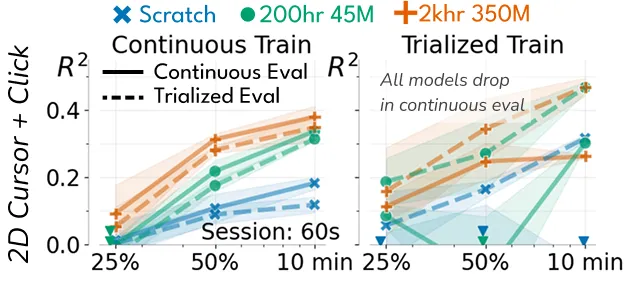
\includegraphics[width=0.7\linewidth]{ch2_trialized.png}
  \caption{Models are evaluated on a human open-loop cursor dataset prepared in two ways.
  Trialized training receives inputs according to trial boundaries, varying from $2$--$4$ seconds in length.
  Continuous training receives random 1 second snippets (that can cross trial boundaries).
  Trialized evaluation matches trialized training, and continuous evaluation is done by streaming up to 1 second of history.
  $\blacktriangledown$ indicates points below 0.0.
  Continuously trained models perform well in both evaluation settings, while models trained on trialized data fail in continuous evaluation.}
  \label{fig:trialized}
\end{figure}
Data efficiency evaluations have shown that NDT3 has learned generically useful priors for predicting motor behavior. We next evaluate generalization to test whether these priors also yield alignment with our normative desires for neural data models. As an example, we show in \figref{fig:trialized} how models trained on trialized data generalize to continuous data.
In this analysis, the training and evaluation data only differ in formatting. Trialized data is segmented and presented to the model so that the model's first and last timestep always coincide with the endpoints of a reaching movement. Continuous data presents random 1 second chops of this same data. \figref{fig:trialized} shows that when trained on trialized data and evaluated on continuous data, from-scratch models degrade substantially while pretrained models only degrade minorly. As desired for BCI control, pretraining may guide models to decode in a more robust and generalizable manner, regardless of neural data formatting.

NDT3’s results are limited in that we only evaluate the specific tokenization mechanism validated by NDT2, and the ratio of data between pretraining and fine-tuning is far smaller than foundation models in other domains, which likely drives the rapid convergence of pretrained and non-pretrained model scores. Nonetheless, it provides a baseline for future improvements, derived from innovations on model design or the next order of magnitude of pretraining data. For deployment to online BCI control, NDT3 clearly provides a better pretrained model than NDT2, though our extended generalization analyses show that our offline evaluations only scratch the surface of aspects of model behavior relevant for online control.



% =========================
% Aim 2
% =========================
\chapter{Aim 2: Pretrained deep networks enable continuous and scalable upper-limb neuroprosthetic control}

\section{Summary and Significance}
Motor cortical BCIs record neural activity that can be used to control a variety of upper limb behaviors, like arm translation, wrist rotation, and hand grasp.
However, this high degree-of-freedom (DoF) control is currently difficult to maintain, requiring daily recalibration and frequent experimenter intervention.
The increased complexity of high DoF BCI control highlights a basic need for BCI models that can be flexibly developed, maintained, and extended.
We propose tuning pretrained NDT3 for this purpose, given its ability to aggregate data of potentially varied formats, from multiple days, into a holistic controller. We will measure NDT3's ability to provide day-over-day performance of 7 DoF, and then 9 DoF control of the upper limb in two human BCI participants. To support this goal, we have conducted pilot assessments of online control. We show that for 2D cursor control, a fine-tuned NDT3 performs comparably with linear baselines, and for 4D virtual limb control combining translation, rotation, and grasp, NDT3 outperforms linear baselines, and improves with data across days.

\textbf{Significance}: This aim assesses whether data aggregation, through its sublimation into the NDT3 model, can meet two critical needs for upper limb neuroprosthetics. First, we assess whether data aggregation can enable continuous and convenient high DoF upper limb control. A reliable and minimally burdensome system is necessary to translate upper limb neuroprosthetics from the lab towards independent device use. Second, we assess whether aggregation is useful to enable the extension of an existing BCI to new behavioral repertoires. If successful, these results would further the case for BCI models that accumulate calibration data across the device's lifetime.

\section{Approach}
We aim to use an NDT3-based deep network controller to enable convenient high DoF control. To this end, our first goal is to enable quick high DoF control across days, by aggregating calibration data across days. Our second goal is to assess the viability of amending and extending control through targeted calibration, primarily by adding more DoF to control.

% Decoders are produced across days through daily recalibration that last upwards of 15 minutes, which imposes substantial calibration burden on the user, and the suboptimal control after this calibration is managed through manual experimenter interventions.
% The development, maintenance, and extension of high DoF movement BCI will require models that can integrate data from multiple days, possibly in varied formats.

\subsection{Rapid calibration on new days}
The requisite time to sample sufficient behavioral diversity to calibrate a high DoF controller grows with behavior dimensionality, reaching 15 minutes for 7 DoF~\citep{collinger2013high} and 20 minutes for 10 DoF~\citep{wodlinger_15_10d}. However, this calibration burden need not be repeated daily, as the relationship between neural activity and behavior only partially changes across days. In speech BCIs and simpler movement BCIs, decoders trained with multiple days of data can be adapted for high performance on new days with minimal, if any, calibration~\citep{sussillo_16_future,hosman2023months,fan2023plugandplay,card2025long}. We aim to replicate this strategy with high DoF motor control.
We will begin these experiments with 30 minutes of calibration in each of the first two sessions.
We will then titer the amount of data we collect for subsequent model maintenance, at a minimum with offline analyses measuring the marginal return on increasing calibration data on new days, and possibly also by directly measuring the amount of continual online tuning needed to reach an 80\% success criteria in our virtual evaluation tasks. We target a final calibration routine of 3 minutes on a new day.
% Why 3 minutes? Justify!

\textbf{Evaluation}: To compare with prior studies, we will evaluate functional performance with timed object transfer trials and the Action Research Arm Test (ARAT), for comparison with prior results in high DoF upper limb control~\citep{collinger2013high,wodlinger_15_10d}. Both protocols assess grasping and carrying competence. To evaluate the continuous stability of system performance, we will target at least 8 experimental sessions over the course of a month. In a subset of these sessions, we will compare against the previous state of the art, 7D control with linear controllers. Due to restrictions on experiment time, comparisons against other baselines and system design choices will use offline prediction-based analyses. In addition to these functional evaluations, we will include a number of virtual brain-controlled reach-grasp-carry sequences in the same setting as the virtual calibration data. These virtual evaluations will allow us to assess more fine-grained control metrics like path efficiency and movement phase-wise performance.

\subsection{Scaling to higher DoF control}
We initially target 7 DoF for robot arm and hand control. For these 7 dimensions, 3 dimensions will be for hand endpoint translation, 3 dimensions will be for wrist rotation, and 1 dimension will control whole hand power grasp. This control scheme has been historically used in our lab and is readily supported by current robot arm and hand capabilities~\citep{collinger2013high}. We will then probe the viability of expanding hand control by changing from 1 DoF power grasp into at least 3 DoF for the hand. We target 2D for thumb flexion/extension and abduction/adduction~\citep{willsey2024real} and 1D for flexion/extension of the other 4 fingers as one group. Depending on our ability to discriminate the other 4 fingers, we may attempt to control them more granularly. We will train and evaluate this new hand control scheme with a focused calibration dataset that varies the hand DoF in isolation, with the arm and wrist in neutral postures. Finally, in preparation for combined control of the hand, wrist, and arm, we will collect a bridging dataset that highlights hand motion in different arm and wrist postures. We expect that minimal calibration in these new postures will suffice to restore performance. For simplicity, we do not plan on collecting calibration datasets where multiple DoF are varying simultaneously.

% Depending on the signal tuning of our new participant, we will at minimum target two additional dimensions of thumb control, or more ambitiously target individual finger control. This minimum is justified in the literature by the robust availability of thumb tuning in several human BCI users implanted near the hand knob~\citep{willsey2024real,shah2025pseudo}. In either case, we will enable this new control with a separate hand-focused calibration dataset. The intent is to demonstrate that a BCI system can accumulate neural-behavior relations in the weights of a deep network, rather than a disparate external collection of datasets. I elaborate on the proposed methods below.
\textbf{Evaluation} Newly attained hand control will be evaluated exclusively in virtual environments. Preserved control of arm and wrist will be evaluated by comparing performance in virtual 7D grasp and carry tasks with and without tuning on the new hand calibration data. If virtual evaluations are successful, we will assess combined arm and hand control with the same ARAT protocol as used to evaluate 7D function. Previous work extending hand control from whole hand grasp into 4 hand-shape basis dimensions~\citep{wodlinger_15_10d} showed that the BCI user preferred not to use the extra dimensions. Thus, the extra dimensions did not provide higher clinical gain of function relative to the 1D whole hand grasp. This may have been a limitation of the linear controllers used at the time or of the control scheme, but given these results, we do not expect higher functional capability with increased hand DoFs.

\section{Results \& Remaining Work}
We have collected pilot experiments that demonstrate the efficacy of NDT3 and its use in multiday aggregation for lower dimensional control, namely for 2D cursor control in three participants and for 4D grasp and carry tasks in Mujoco with one participant.

\begin{figure}[h]
  \centering
  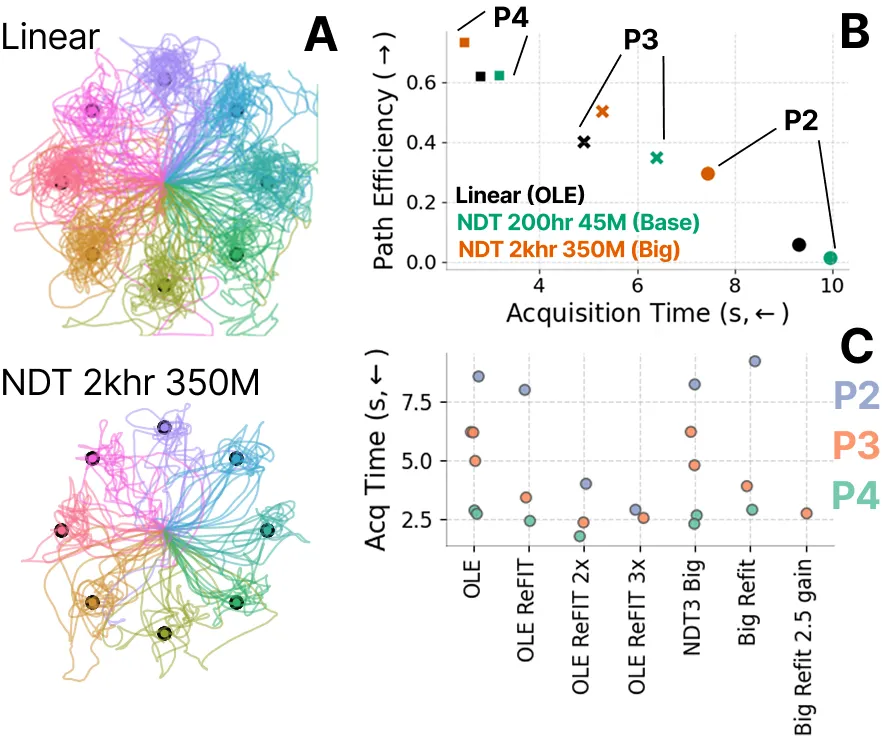
\includegraphics[width=0.8\linewidth]{ch3_cursor_control.png}
  \caption{A. OLE and NDT brain-control trajectories in one human participant. B. The largest NDT model matches linear model performance for 2D cursor control when all models are trained on an open loop calibration block. B. With closed loop tuning, linear control steadily improves, but NDT does not. This gap can be closed by increasing NDT's gain manually.}
  \label{fig:cursor}
\end{figure}

\textbf{2D Cursor control}: We have compared NDT3 against linear controllers for 2D cursor control with three participants, each in two separate sessions. These controllers are directly created from training on open loop calibration data alone, without further closed loop tuning. Qualitatively, the NDT3 model often produces slower, steadier movement compared to the linear controller~(\figref{fig:cursor}A), whereas quantiative measures of path efficiency and acquisition time show rough similarity between the linear baseline and NDT3 models~(\figref{fig:cursor}B). Given the qualitative difference in control, we note that this measured equivalence likely depends on the particular distance and precision requirements in our evaluation task~\citep{willett2017comparison}.

Cursor controllers are often adapted after blocks of closed loop control to improve performance~\citep{jarosiewicz2013advantages,gilja2012high,willett2017comparison}, and so evaluating models after blocks of closed loop tuning likely better reflects real world performance limits. We use the ReFIT intention estimation strategy~\citep{gilja2012high} to enable closed loop adaptation of both linear and NDT controllers. We replicate that control reliably improves with ReFIT across participants, but that NDT control does not improve as significantly~(\figref{fig:cursor}C). NDT does not benefit as greatly from reducing angular decoding errors and experiences a degradation in control gain. Observing this, we observed greatly increased performance from manually increasing NDT gain. We speculate that NDT suffers more significantly from the label noise introduced across the multiple calibration datasets. This result motivates care in the use of closed loop tuning for NDT. We do not anticipate this result to prohibit our high DoF study, as historical high DoF experiments were reported without intention estimation, and closed loop tuning does not majorly affect performance in our most recent participant with the highest signal quality recordings (P4), which is the setting we will study for high DoF control.

\begin{figure}[h]
  \centering
  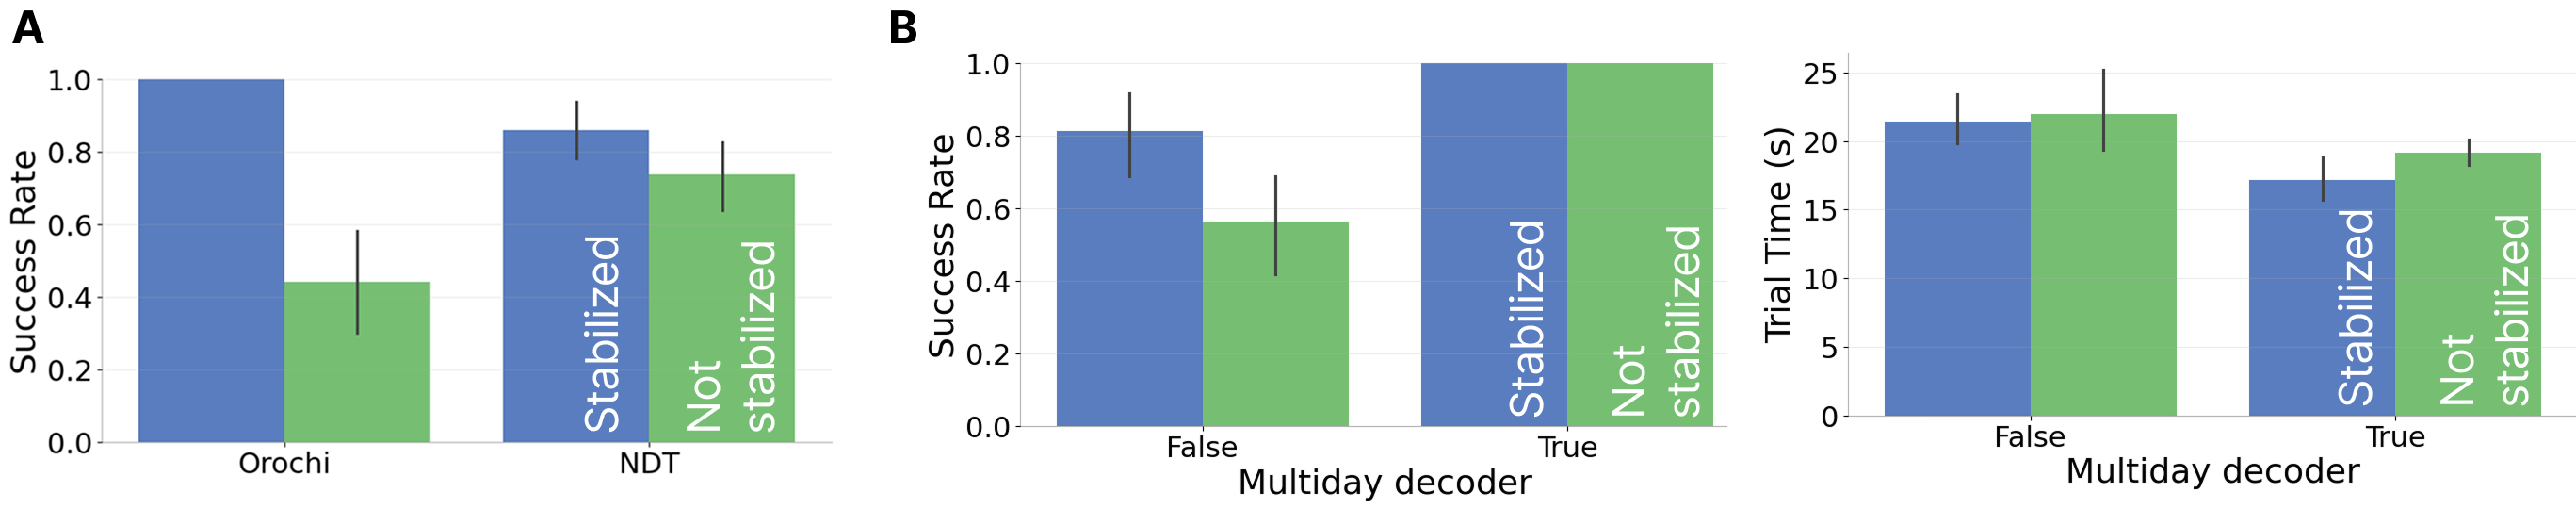
\includegraphics[width=1.0\linewidth]{ch3_mujoco_results.png}
  \caption{A. Orochi linear decoder compared against NDT DNN decoder for Mujoco 4D FBC Sequenced movement trials. Error bars show standard deviation across trials. Evaluations are conducted in default (not stabilized) and stabilized settings. Stabilized evaluations only allow one of arm translation, wrist rotation, or hand grasp to be active at a time. B. Multiday NDT decoders achieve high success and faster completion times relative to decoders trained from scratch.}
  \label{fig:mujoco}
\end{figure}

\textbf{4D Mujoco control}: We have also collected several sessions of 4D control, with 2 arm translation dimensions, wrist roll, and whole hand grasp, calibrated and evaluated in the Mujoco simulator. All trials are sequenced movement tasks that have distinct phases that require isolated translation, rotation, and grasp. These experiments derisk two aspects of DNN control we target in our high-DoF experiments.

First, NDT provides distinctive stability benefits for high-D control. By stability, we specifically mean it is hard for the virtual effector to remain on target for a sufficient holding period to pass the trial. This failure mode degrades the linear decoder in regular evaluations where all DoF are allowed to vary in all phases, despite good performance in a stabilized evaluation where irrelevant DoFs are frozen in each phase. This lack of stability is a known phenomena of linear models and has motivated prior works to explore nonlinear output scaling for 2D cursor control to enable easier stopping~\citep{sachs2015brain,card2025long}.
The increased severity of instability at higher dimensions has not been saliently discussed in prior works, perhaps because no alternative was available at the time. In contrast with linear decoders, NDT does not suffer a large performance drop from removing movement constraints, due to its inherent minimal movement in off-target dimensions. This stabilizing aspect of DNNs is corroborated in DNN-enabled 4D bimanual control~\citep{deo_23_impulse}, and suggests that DNNs like NDT will provide qualitatively superior control over linear controllers in high dimensions due to a tendency of DNNs to isolate DoF, despite their quantitative similarity for cursor control. For clarity as to why this happens, we can turn to two monkey studies~\citep{temmar2024artificial,costello2023balancing} that suggest that RNN decoders will tend to more precisely replicate training label distributions, which in our case have isolated translation, rotation, and grasp. This result does raise the potential of requiring calibration that varies multiple DoF simultaneously, though that has not yet limited our 4D brain control experiments.

Second, NDT supports multiday adaptation for arm and hand control. \figref{fig:mujoco}B shows these brief multiday results for 4D, showing 2 evaluation days where the NDT decoder had either 2 or 3 days of full calibration data. Thiese multiday decoders enjoy a moderate performance gain by both success rate and acquisition time. We take this as evidence that a multiday NDT decoder will likely sustain a fixed level of performance with reduced calibration data.

The main high-D experiments have not yet begun. The main set of proposed experiments will likely only be viable to test with a new participant we expect to implant in late August due to array degradation or participant health in our other participants. We must first show that we can achieve day-over-day 7D control for Mujoco environments and robot arm control, and that the stated stability properties are beneficial for functional tasks. We target demonstration of sustained control for up to a month. Conditions permitting, we will try to enable sustained 7D control for a second participant with arrays that are 2 years old. I will then target finger control calibration and evaluation, anticipating around 6 sessions of data collection.

% I may also pursue technical improvements in the decoder that will improve performance, without changing the main study design or endpoints described thus far. Two directions of interest are new strategies for closed loop decoder tuning, for reasons described in the cursor experiments, and the integration of external priors from pretrained behavior models.

% =========================
% Aim 3
% =========================
\chapter{Aim 3: Modeling the neural response to intracortical microstimulation}


\section{Summary and Significance}

% \begin{figure}[h]
%   \centering
%   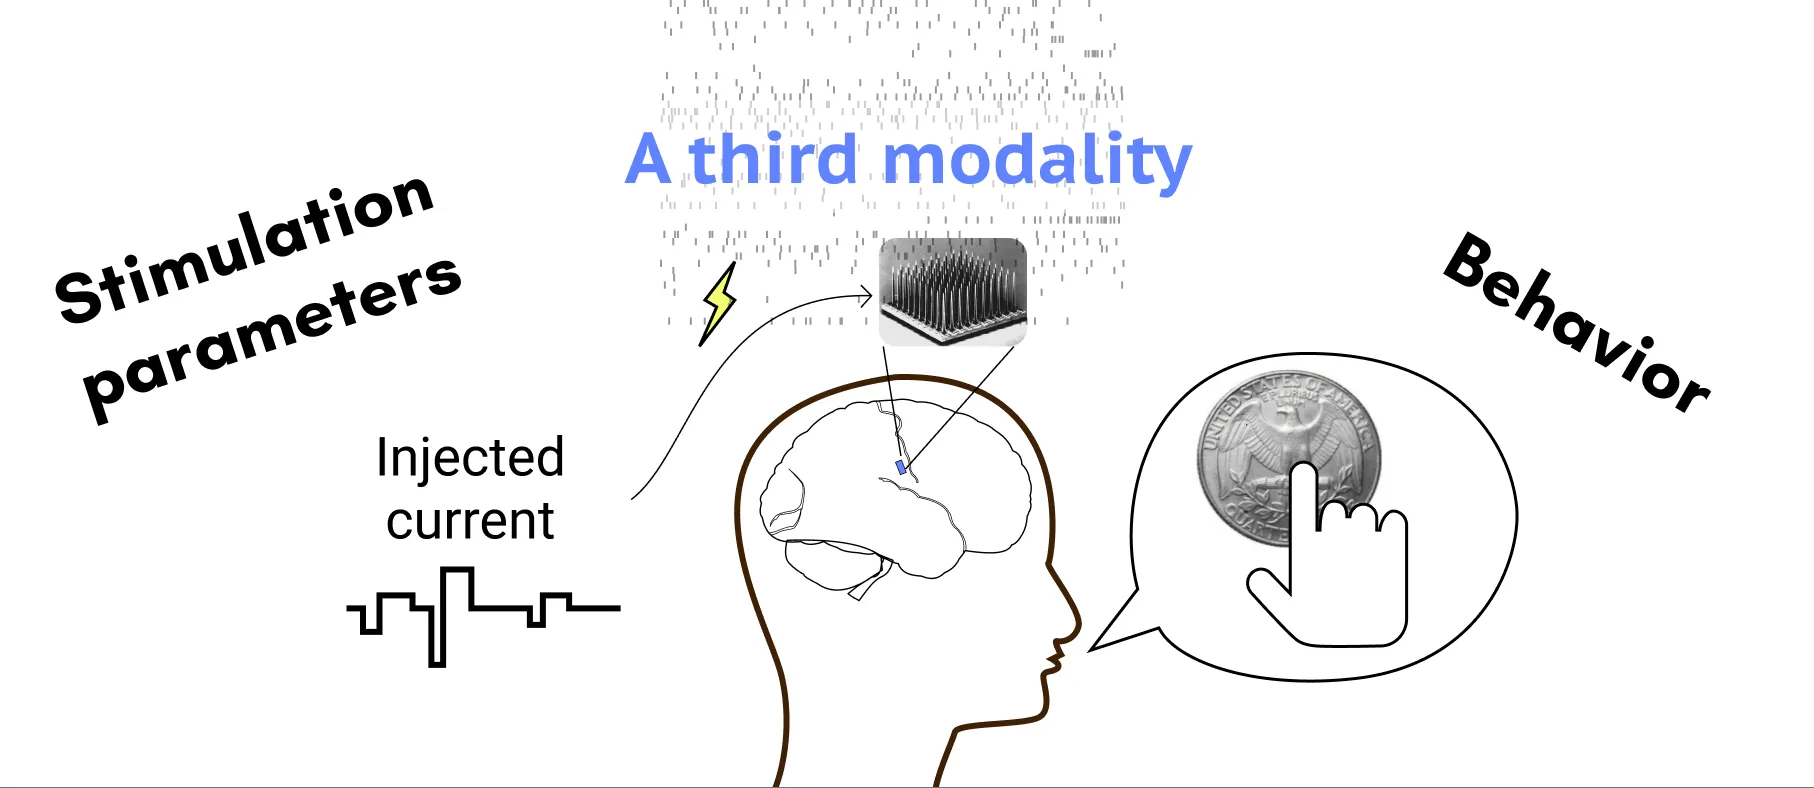
\includegraphics[width=0.5\linewidth]{ch4_third_modality.png}
%   \caption{Third modality analysis for ICMS modeling.}
%   \label{fig:third_modality}
% \end{figure}
Today’s neural interfaces provide the ability to intervene on ongoing neural activity through stimulation. This ability can be valuably applied in intracortical BCIs to provide sensory information about the user’s environment. The evoked sensory response to different stimulation parameters can be characterized and composed in simple manners to convey basic tactile features, and integrated to improve grasping efficiency~\citep{flesher2021functional,valle2025tactile}. The challenge is to now advance beyond this initial characterization and to more thoroughly relate the exponentially large and artificial parameter space of electrical stimulation patterns to the high dimensional and qualitative space of sensory perception.

% Could use some citations throughout... but IDK
To enable a data-driven approach for this challenge, we must augment stimulation characterization beyond the current norm of noisy and slow perceptual reports. This can be done by decomposing the current stimulation modeling problem into two: relating stimulation and the evoked local neural response, and relating the local neural response and subsequent percept. This decomposition strategy relies on two critical assumptions. First, given the spatiotemporal locality of the immediate neural response to ICMS~\citep{eles2021temporal,kumaravelu2022stoney,kumaravelu2024neural}, we assume that the controllable variability in the subsequent perceptual response to stimulation is mediated by the locally observed neural response. Second, to scale data collection for the neural response model, we assume that the neural and perceptual response to passive task-free stimulation is informative of the response in functional task contexts. With these assumptions, we also defer the challenge of relating the neural response to perceptual response, and focus in this proposal on two challenges in modeling the local neural response to passive stimulation.

First, we introduce a new method for electrical artifact removal that allows the recovery of spiking activity on the stimulating electrode array, where neural responses relevant to the perceptual report are likely to be. Second, we characterize how the neural response to different spatiotemporal stimulation patterns relate to each other, under the lens of transfer learning. We identify that responses remain largely predictable under temporally varied stimulation, but responses across different channels are idiosyncratic. These results inform a strategy for accumulating a model of the neural response to stimulation through passive stimulation.

\textbf{Significance}: Modeling the neural response to stimulation may provide a critical foothold to developing sophisticated intracortical stimulation strategies. Our artifact removal method enables this, by enabling the recovery of short-timescale neural responses. The latter study, which aims to taxonomize the neural response to passive stimulation, provides basic recommendations for how to build a tractable model of the neural response to stimulation. The utility of such a model will rest on the strength of the relationship between the neural and perceptual response. For example, our neural taxonomy identifies channel specific idiosyncrasies in the neural response to ICMS, which is also reported at the level of behavioral response~\citep{greenspon_25_stable,hughes2021perception}. If the two phenomena can be connected, it would imply our neural response model should greatly inform our ultimate functional goal of modeling the perceptual response to stimulation.

\section{Approach}
\subsection*{Recovering the neural response with DELETE}
The first obstacle to modeling the neural response to stimulation is simply observing the neural response to stimulation. The hardware required to enable simultaneous electrophysiological recording through stimulation has only recently arrived in NHP and human labs, and on these hardware, large electrical artifacts will often distort the putative spikes extracted by conventional signal processing. The artifacts induced in our experimental setup are particularly severe and warranted the development of a new artifact rejection approach which we call DELETE (Denoising Electrical Events with a Transformer Encoder). DELETE is a nonlinear generalization of population reconstruction-based methods including ERAASR~\citep{oshea2018eraasr} and linear regression rereferencing (LRR)~\citep{young2018signal}.  We will show that DELETE outperforms these methods and other baselines both in recovering peri-stimulation neural responses and in generically denoising broadband activity.

\begin{figure}[h]
  \centering
  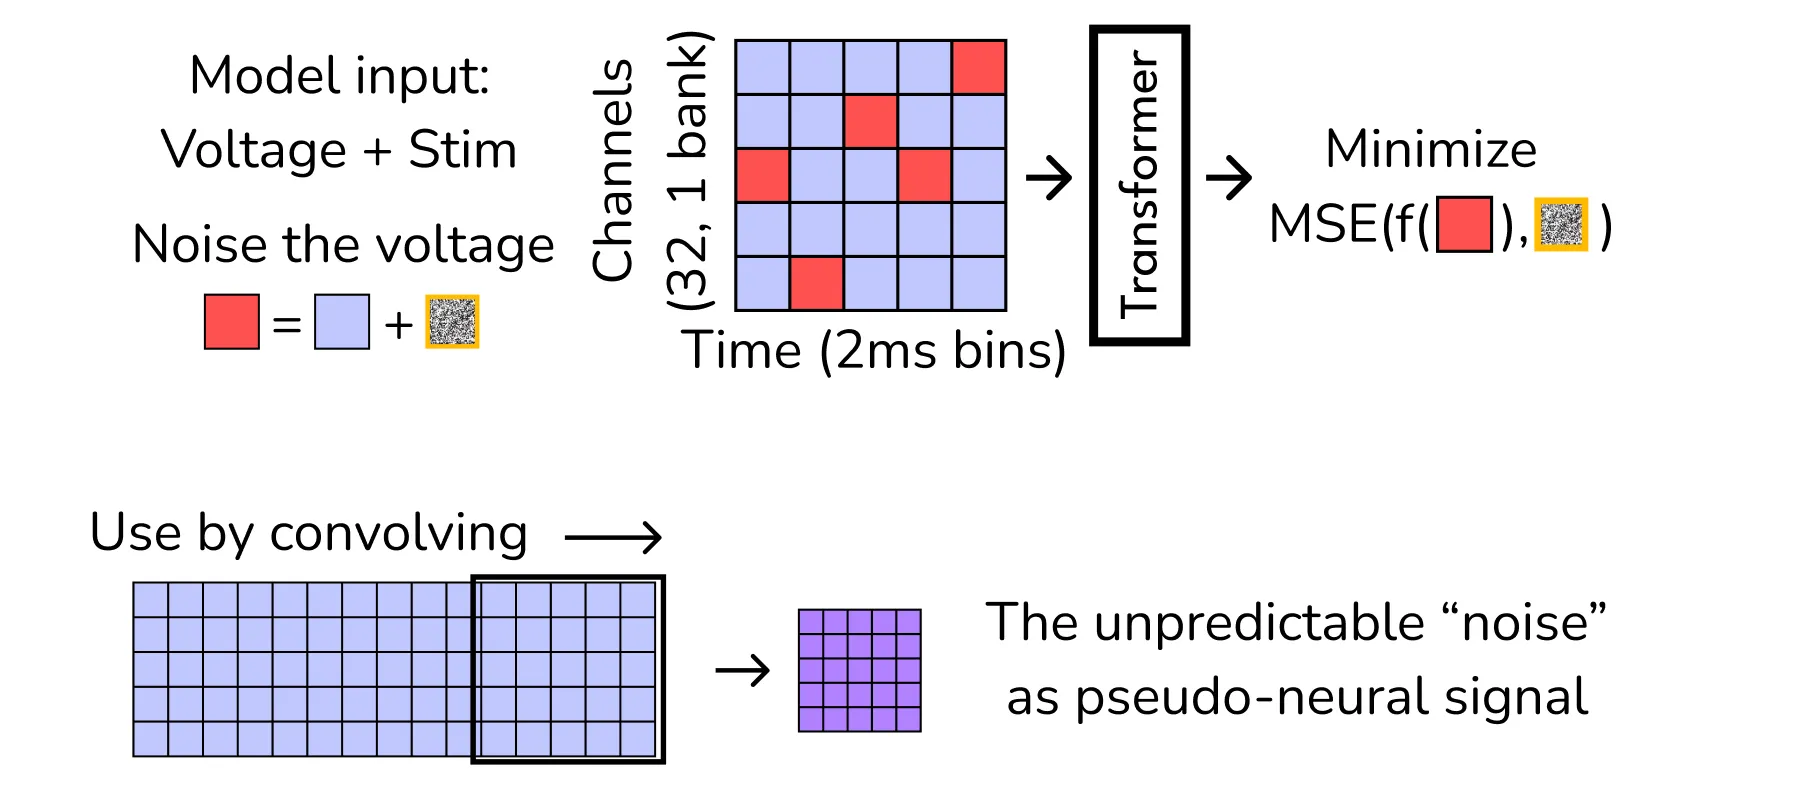
\includegraphics[width=0.8\linewidth]{ch4_delete_schema.png}
  \caption{DELETE schematic. DELETE is a denoising autoencoder that is optimized to predict the noise component of data that has been injected into fractions of its input. At test time, DELETE is applied by convolution on raw broadband activity, and the model's predicted noise components form putative de-artifacted, neural signal.}
  \label{fig:delete_schema}
\end{figure}


\textbf{DELETE Design}: DELETE is a deep network optimized to reconstruct broadband multichannel neural activity. Reconstructed activity is assumed to be artifact due to its rough similarity across channels, and subtracted to recover putative neural activity. While similar reasoning has motivated previous PCA-based methods~\citep{oshea2018eraasr}, DNNs have renown as universal function approximators, which makes it unclear whether DELETE might also reconstruct and remove neural activity in addition to electrical artifact. We rely here on info-theoretic intuitions to constrain DELETE’s behavior, restricting its input window (e.g. 6 ms) and forcing its training across broad data under a point-estimate loss (mean-squared error). Combined, these restrictions imply a network could only erase neural activity by knowing the precise firing characteristics of a specific channel when deployed on an arbitrary new 6 ms window. Ultimately, like other artifact rejection methods, DELETE is best justified empirically, from our broad validation.

DELETE joins a number of related methods using deep learning to process raw scientific data~\citep{wang2023scientific}. DELETE relates to the use of autoencoding for anomaly detection to remove uninteresting background events, as in e.g. particle collision experiments, so as to highlight the residual signal. DELETE critically should be distinguished from similar-sounding denoising autoencoders~\citep{lecoq2021deepinterpolation,liu2025astro_denoise}, which \textit{preserve} the common component of multidimensional data and discard the residual as noise. Beyond this distinction in usage, DELETE is distinguished in design by its use of Gaussian noise to ease the learning of the task, as the artifact is otherwise too variable for satisfactory estimation. The model does not use fully masked inputs to directly reconstruct broadband activity, but rather receives input activity distorted by additive Gaussian noise, and must predict the injected noise.

\textbf{Analysis}: Our analysis of the DELETE method has three components. We first evaluate its performance as a stimulation artifact rejector, focusing on activity recovered in short periods after stimulation pulses. This analysis will be performed on a variety of ICMS datasets, discussed further in the next section. We next evaluate its performance as a generic denoiser, using synthetically noised datasets and datasets with movement artifacts. Finally, we conduct isolated studies of model behavior over input and architectural ablations, to build an understanding of model function.


\subsection*{Taxonomizing passive ICMS responses}
To productively scale data collection to model the neural response to ICMS, we must first build a coarse understanding of the impact of different stimulation parameters. The full parameter space is exponential, but the presence of some structure in the behavioral response to ICMS suggests that there are natural axes of data diversity in the neural response as well. Thus, we taxonomize which sets of ICMS parameters evoke structurally similar responses, by collecting datasets of passive ICMS stimulation and observing how models (RNNs or Transformers) trained on one subset of the data generalize to other subsets~\citep{zamir2018taskonomy}. We first collect multiple single electrode ICMS datasets that vary pulse timing and amplitude, either using the fixed parameter trains commonly used in ICMS protocols to date, or with random amplitudes and Poisson timing. We also collect corresponding single and multi-channel datasets to assess whether we can back out performant models of single channel stimulation from multi-channel datasets. Finally, we scale spatiotemporally randomized multichannel stimulation trains over months to illustrate that multiday models can productively accumulate these diverse data, similar to our strategy for motor models.


\section{Results \& Remaining Work}
Thus far we have trained and evaluated the DELETE estimator on ICMS datasets using both simple, single-channel fixed frequency and amplitude trains and multi-channel, spatiotemporally diverse trains. The taxonomy project has proceeded under the assumption that DELETE has properly de-artifacted our ICMS datasets. The requisite passive ICMS datasets were collected in 2022 to 2023, in 2 participants.

\begin{figure}[h]
  \centering
  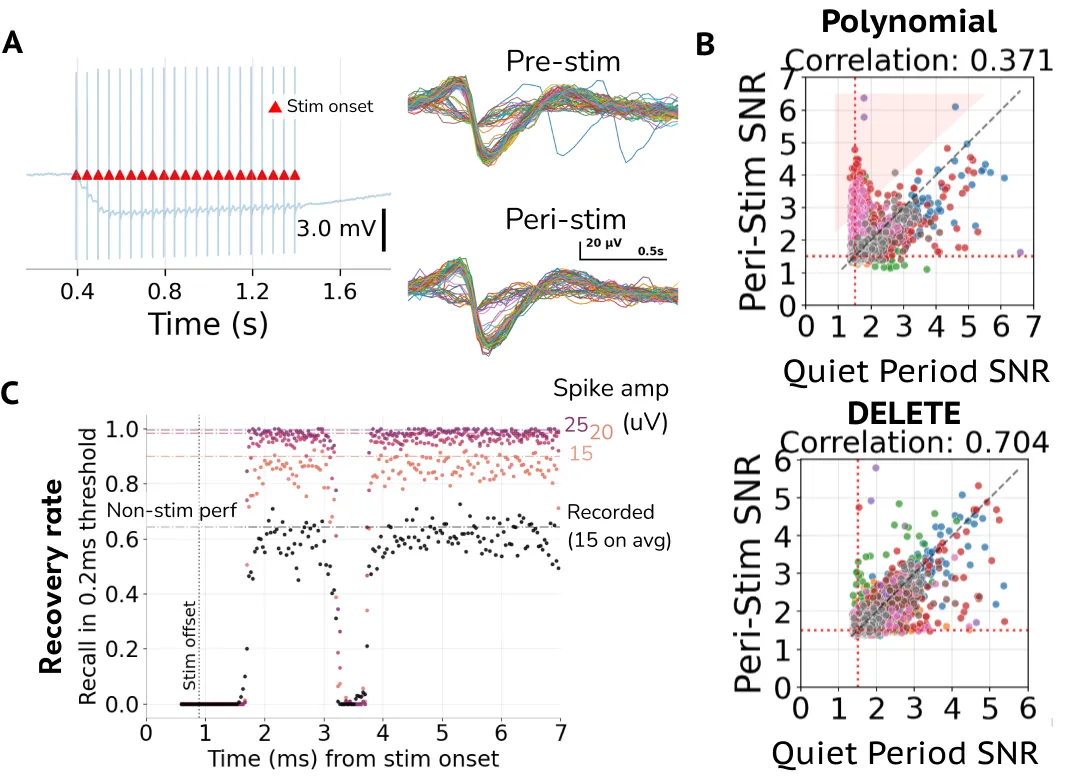
\includegraphics[width=0.8\linewidth]{ch4_delete_peristim.png}
  \caption{A. Left: A sample broadband recording from a channel during a stimulation trial. The displayed channel is on the electrode array that is stimulated. Right: Spike waveforms recovered from the broadband activity both prior to stimulation onset and in the artifacted peri-stimulation period. B. To summarize waveform recovery, we compute channel SNR as a ratio of peak waveform amplitude against background noise amplitude. The color of each dot indicates the physical array the channel is on. We expect physiological waveform SNRs to be conserved through stimulation, so high correlation of quiet period and peri-stim SNR provides a heuristic for good de-artifacting. Dashed red lines indicate the 4.5x background noise threshold we use to determine spike presence. C. We evaluate model sensitivity by injecting synthetic spikes into the broadband activity and evaluating whether they are recovered. The colored curves differ in the precise waveform injected, which were either recorded and extracted from the data or simulated. Horizontal lines indicate the noise ceiling computed as the recovery rate of spikes injected outside of stimulation periods.}
  \label{fig:delete_peristim}
\end{figure}


\textbf{DELETE for ICMS artifact rejection}: As we began passive ICMS data collection, we quickly observed stimulation artifacts in our data that were more severe than those typically seen in the literature. Specifically, our stimulation induces not only a large, high amplitude transient on each stimulation pulse, but also includes a post-transient distortion that decays on the timescale of a second~(\figref{fig:delete_peristim}A). Our task is to remove this artifact so as to extract the neural spiking activity. Ideally, the extracted spiking activity will be verifiable based on the spike’s waveform shape, though this may be challenging given that the spike is typically much smaller in amplitude than even the artifact’s slow decay. An example of a channel with one distinctly preserved waveform is shown to the right. The challenge is to do this reliably, across stimulation parameters and channels. In \figref{fig:delete_peristim}B, we show example waveform recovery summaries from a single stimulation dataset for two different artifact estimation methods. Polynomial estimation has many high amplitude waveforms recovered in peri-stimulation period, even for otherwise very quiet channels, due to artifact leakage. We seek methods that have high correlation across channels and datasets, and DELETE greatly outperforms the other baselines we have developed. In \figref{fig:delete_peristim}C, we show an synthetic sensitivity analysis computed on a dataset processed by the DELETE method. To create these recall curves, we injected synthetic spikes into broadband activity at different offsets from a stimulation pulse onset. We prohibit spike recovery shortly after each pulse and in a timeframe around 3ms after each pulse due to high artifact severity, but outside of these blanked periods, nearly all injected spikes are recovered. We can compute area-under-curve metrics for different methods in this analysis, and DELETE typically outperforms baselines here as well.

\begin{figure}[h]
  \centering
  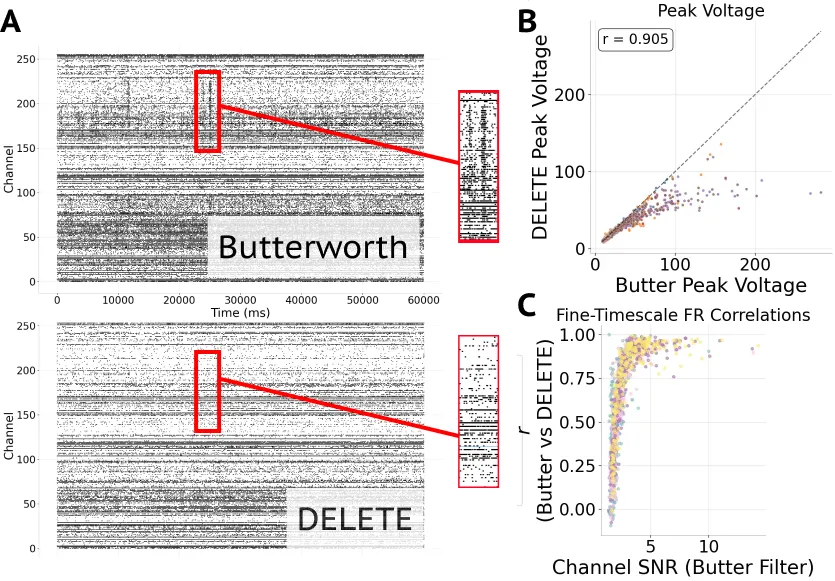
\includegraphics[width=0.8\linewidth]{ch4_delete_generic.png}
  \caption{A. Top: Butteworth filter extracted spiking activity from a minute of resting state recordings. Inset shows putative movement-induced artifact. Bottom: The same data pre-filtered by DELETE, inset no longer shows correlated firing across channels. B. Peak voltages of waveforms extracted by DELETE and a standard Butterworth filter are compared. There is high correlation, but DELETE peaks saturate by 100$\mu$V. C. Firing rates are determined by convolving a 50ms Gaussian kernel against Butterworth or DELETE filtered spiking activity. These per-channel firing rates are correlated across a number of different channels and datasets. Color of dots indicate datasets. High SNR channels correlate well.}
  \label{fig:delete_generic}
\end{figure}

\textbf{DELETE as a generic denoiser}: DELETE is a method that convolves over all timepoints and therefore applies to non-stimulation datasets as well. Its objective implies it may be a useful generic denoiser to remove non-neurophysiological signals that degrade our recordings, so we try to characterize this intuition in~\figref{fig:delete_generic}. In panel A we show two raster plots computed from the same minute of resting state activity recorded from one of our BCI participants. The Butterworth filtered data show several streaks of transient high firing across multiple channels that typically indicate electrical noise caused by participant movement. The DELETE pre-filter produces an overall quieter view of this same activity, and notably also does not contain these periods of correlated firing.

The broad change in statistics may be concerning, but similar changes can occur even as the result of changing classical filter settings. We still cannot evaluate against any underlying ground truth, but we can rely on the principle that the activity of high amplitude and therefore high quality spikes should be well conserved. \figref{fig:delete_generic}B and C show that DELETE does satisfy this requirement. B shows that DELETE roughly conserves the peak voltage of spike waveforms, so large spike waveforms will remain large regardless of DELETE pre-filtering. There is a notable saturation in DELETE-processed waveforms at around 100$\mu$V, which likely corresponds to the amplitude of the noise used in DELETE’s training. We can also show that single channel firing is conserved at a more detailed level, by correlating the firing rates identified with or without the DELETE pre-filter. In doing so, we see that as hoped for, high SNR channels again have highly conserved firing rate timecourses.



\begin{figure}[h]
  \centering
  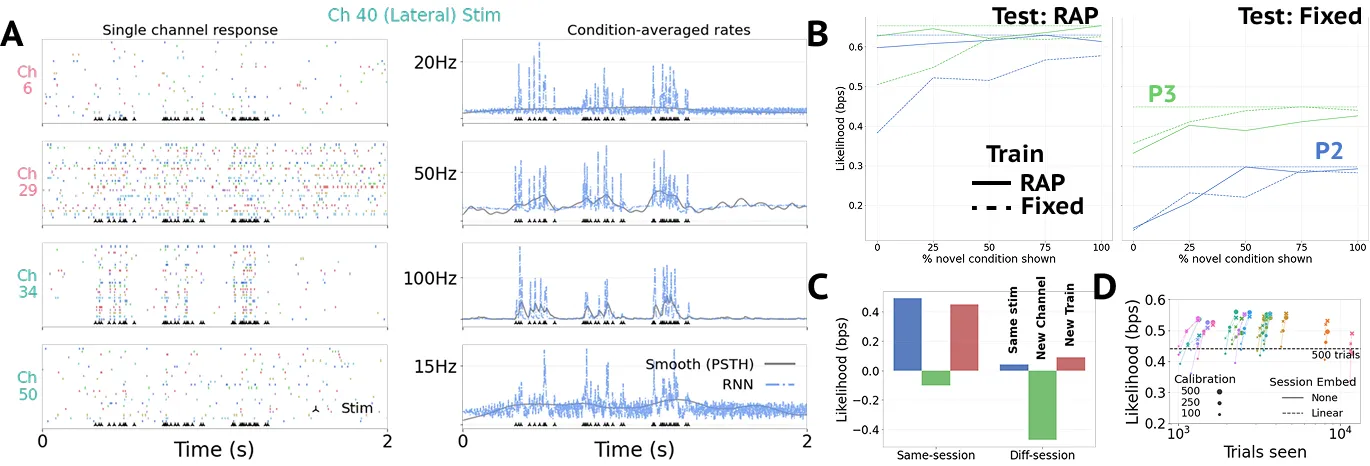
\includegraphics[width=1.0\linewidth]{ch4_icms_taxonomy.png}
  \caption{A. Example rasters to stimulation on a single channel (40). Modulated responses are visible both on the stimulated array (bottom two rows) and another sensory array (top two rows). Firing rates as inferred by computing PSTH and RNN models are given on the right. B. Example analysis testing generalization of RNN models to novel single channel stimulation trains. In these plots, models are first trained on either random amplitude Possion (RAP) or fixed frequency and amplitude trains (Fixed). They are then gradually exposed to increasing levels (\% novel condition shown) of a new set of ICMS again from either RAP or fixed stimuli (Test condition). The flat dotted line marks the max performance achieved by any in-distribution model. The closer the other curves are to this flat line, the better the model's generalization to new stimuli. C. We train one model on one type of RAP ICMS and assess its generalization to 3 stimulation conditions from either the same or different experimental session. D. We conduct a brief scaled pretraining analysis. We vary the pretraining scale (Trials seen) and subsequent fine-tuning scale (Calibration), and evaluate on a new session. Session identity is either not modeled (Session Embed None) or modeled with a linear readin layer (Linear). The reference line shows session performance using only 500 calibration trials from the evaluation dataset. Most pretrained models exceed this level, suggesting positive transfer.}
  \label{fig:icms_taxonomy}
\end{figure}

\textbf{ICMS Taxonomy}: To characterize how the neural response to different ICMS trains relate to each other, we collected a variety of ICMS datasets and modeled them with RNNs (chosen for efficacy at very small data scales). This flexible model-based characterization of data relationships are necessary as we are interested in the response to spatiotemporally diverse ICMS, as opposed to only fixed parameter trains. One such temporally varying ICMS train is shown in~\figref{fig:icms_taxonomy}A. Modulated responses on both stimulated and non-stimulated arrays can be modeled with an RNN model. Panel B shows an example generalization assay that tests whether models trained on data from one family of ICMS data will generalize to another. Responses to random-amplitude poisson (RAP) trains are well-predicted if models have already trained with other RAP trains, but generalization to unseen fixed parameter trains is poor regardless of whether the model has first trained on RAP or fixed parameter ICMS.
We have run a number of similar analyses testing generalization across stimulation channels and timing, and tentatively believe that RAP trains provide a good basis to learn the broad response to stimulation on a given channel, but there appears to be little correspondence between the evoked response on different channels. The next two panels address model generalization across days. \figref{fig:icms_taxonomy}C first restates that generalization to repeats (Same stim) and to new RAP trains (new train) is high, but generalization to new channels is poor. The same relative ordering holds when the data is collected from a different experimental session, but all scores are greatly reduced. \figref{fig:icms_taxonomy}D shows that despite this session-wise drift, we can train an RNN model on increasing volumes of ICMS data to achieve high model performance on new days. The decline in performance at the high end of pretraining scale currently challenges a straightforward ICMS foundation model built with RNNs, and prompted the long detour to develop multisession modeling capability with the NDT models. We have yet to assess whether NDT models scale resolve these scaling difficulties.

The remaining work for DELETE is to polish the existing per-dataset profiles into a summary of DELETE’s efficacy. This entails characterizing a polynomial estimator baseline and linear regression rereferencing, and developing a synthetic battery. We also aim to ground DELETE’s performance in plausible neurophysiology. We can verify this for the generic denoising case by applying DELETE to motor datasets and verifying it conserves population structure and decodable information. For the ICMS case, we will check that DELETE’s recovered distribution of evoked responses resembles those from external datasets collected in settings without our severe artifacts.

The taxonomy work is in a similar state, where the technical proof of concept is nearly complete, but the analysis needs extension to many datasets. As we already have one more participant and may soon have another, we may consider further data collection to improve the strength of our conclusions. For example, to strengthen the relevance of this study to rehabilitative BCI, we should demonstrate whether the fully passive data collection protocol also generalizes to data collected in functional (but non-motoric) tasks where participants must report sensation. Beyond this, I see three possible directions to extend the work: generalizing the findings by extending the analysis to new brain areas (e.g. V1 or PFC, by collaboration), translating the model for ICMS control by developing an inverse model, or grounding the response in sensory experience by using it to decode participant reports. I have left time in my schedule in Q2 2026 to allow these potential extensions.


% =========================
% Schedule
% =========================
\chapter{Schedule}
I began my doctoral research with a stimulation focus (Aim 3), but put it on hiatus to study how we might aggregate neural datasets (Aim 1). My remaining schedule begins with data collection for NDT-control experiments (Aim 2). As those experiments wind down I expect to be able to focus on writing those results up while running analysis and writeup for Aim 3. Note I expect Aim 3 to produce two publications, one on the artifact removal work and one on the ICMS response taxonomy work.

\begin{figure}[h]
  \centering
  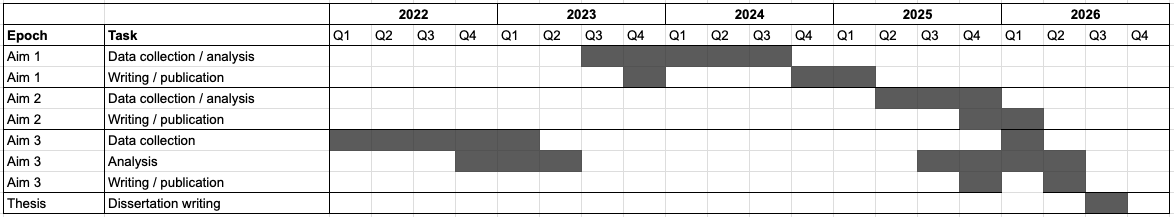
\includegraphics[width=1.0\linewidth]{ch5_schedule_gantt.png}
  \caption{Gantt chart overview of project priorities throughout the PhD.}
  \label{fig:schedule}
\end{figure}

% =========================
% References
% =========================
\cleardoublepage
\printbibliography

\end{document}
